\documentclass{article}
\usepackage{standalone}
\usepackage{tikz,pgfplots}
\pgfplotsset{compat=1.10}
\begin{document}
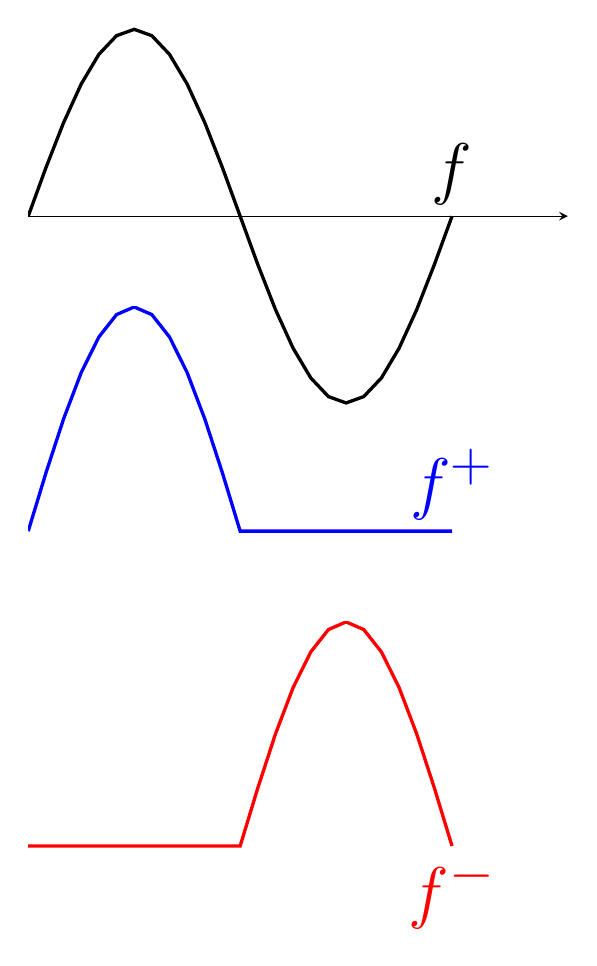
\begin{tikzpicture}
    \begin{scope}
	\begin{axis}[ticks = none,axis x line=center,hide y axis,xmax = 8]
	    \addplot[domain=0:2*pi,black,very thick] {sin(deg(x))} node[above,pos=1] {\Huge$f$};
	\end{axis}
    \end{scope}
    \begin{scope}[yshift=-4cm]
	\begin{axis}[ticks = none,axis x line=center,ymin=-1,ymax=1,hide y axis,hide x axis,xmax = 8]
	    \addplot[domain=0:2*pi,blue,very thick] {x > pi ? 0 : sin(deg(x))} node[above,pos=1] {\Huge$f^{+}$};
	\end{axis}
    \end{scope}
    \begin{scope}[yshift=-8cm]
	\begin{axis}[ticks = none,axis x line=center,ymin=-1,ymax=1,hide y axis, hide x axis,xmax =8]
	    \addplot[domain=0:2*pi,red,very thick] {x < pi ? 0 : -sin(deg(x))} node[below,pos=1] {\Huge$f^{-}$};
	\end{axis}
    \end{scope}
\end{tikzpicture}
\end{document}
